\documentclass{article}

\usepackage{amsmath}
\usepackage{amsthm}
\usepackage{amssymb}
\usepackage{mathtools}
\usepackage[a4paper, total={7in, 10in}, headheight=0pt, headsep=0pt]{geometry}
\usepackage{titling}
\usepackage{hyperref}
\usepackage{graphicx}

\newcommand{\Z}{\mathbb{Z}}
\newcommand{\mi}{\text{mid}}
\newcommand{\up}{\text{Up}}
\newcommand{\down}{\text{Down}}


\newcommand{\pav}{Pálvölgyi}
\setlength{\droptitle}{-6em}


\renewcommand{\qedsymbol}{$\blacksquare$}

\begin{document}
    For $N, d \in \Z_{\geq 1}$ let  $L = [N]^d$ be the $d$-dimensional integer lattice with height $N$ under coordinatewise ordering $\leq$, and $f: L \to L$ be
   a monotone function on $L$. So if $l, l' \in L$ with $l \leq l'$ then $f(l) \leq f(l')$. 
   Our goal is to find a fixpoint of $f$. That is, an $l^* \in L$ such that $f(l^*) = l^*$.\\

  Let $a \leq b \in [N]^d$. Then define $L_{a, b} = \{ l \in L : (a_1, ..., a_d) \leq l \leq (b_1, ..., b_d) \}$ 
  to be a subset of $L$.
  It is clear that $L_{a, b}$ is also a lattice under the same ordering. \\

  The strategy currently under consideration is an extension of the algorithm found in
  the paper from Fearnley, Pálvölgyi, and Savani\cite{FePaSa}, which is itself similar
  to an algorithm originally given by Dang, Qi, and Ye\cite{DangQiYe}. \\

  The core idea
  in the Dang, Qi, and Yi algorithm is that if $l = (l_1, ..., l_d)$ satisfies
  $f(l)_i = l_i$ for $i \in \{1, ..., d-1\}$ then either $f(l)_d \geq l_d$ or $f(l)_d \leq l_d$.
  In both cases $f$ restricts to a sublattice where the $d$th dimension is restricted to points
  above or below $l_d$ if $f(l)_d \geq l_d$ or $f(l)_d \leq l_d$ respectively. There
  is then a natural recursive algorithm that chooses the midpoint $\mi_d = \frac{b_d - a_d}{2}$ in the $d$-th dimension,
  recursively finds a fixpoint $\overline{l}$ of the $d-1$ dimensional slice at $l_d = \mi_d$, then 
  depending on if $f(\overline{l})_d \geq \overline{l_d}$ or $f(\overline{l})_d \leq \overline{l_d}$,
  recurse on the half-lattice above/below $l_d$ in the $d$-th dimension. In the one-dimensional base-case,
  one dimensional binary search can give you a fixpoint in $\log N$ time, so this algorithm takes
  $O(\log^d N)$ time.\\

  
  Fearnley, \pav, and Savani made the observation that a fixpoint of the $d-1$ dimensional slice is not required; 
  a point $l = (l_1, ..., l_{d-1}, \mi_d)$ such that either $f(l)_i \leq l_i$ for all $i \in \{1, ..., d\}$ or 
  $f(l)_i \geq l_i$ for all $i \in \{1, ..., d\}$ is sufficient to restrict to a half-lattice. Further,
  they gave an algorithm - coined the 'inner-algorithm' - which can find
  such points in the 3 dimensional problem in $O(\log N)$ time. This leads to an algorithm which
  can solve the $d=3$ case in $\log^2 N$. There are also decomposition theorems that show these faster
  low-dimensional algorithms can be used to solve the problem in higher dimensions faster than
  the Dan, Qi, and Ye algorithm. \\

  My current work is on designing an algorithm which can solve the 4 dimensional problem in $\log^2 N$ time.
  In particular, I am trying to build on the idea of Fearnley, \pav, and Savani in designing an inner-algorithm
  which can given a fixed value $\mi_4$ in the 4-th dimension find a montone point 
  $(l_1, l_2, l_3, \mi_4)$ in $O(\log N)$ time. \\

  One iteration of the inner-algorithm looks roughly as follows. (The paper details an earlier preprocessing step,
  but I neglect this for now.)
  \begin{itemize}
    \item there is an inductive invariant maintained throughout the runtime of the algorithm;
      \begin{enumerate}
        \item there is a pair of points $(a, u), (d, b) \in L^2$ on the edge of the square.
        \item these points guarantee the existence of a monotone point in the instance
      \end{enumerate}
    \item query the mid point of the square slice
    \item query one more point dependent on the result of the midpoint query
    \item based on this information, we have either an immediate solution to the
      inner algorithm, or a new pair of points on one of the lines through
      the centre of the square which can replace $(a, u)$ or $(d, b)$, allowing
      us to half the search space.
  \end{itemize}



  Consider the case $d=4$, let $l = (l_1, l_2, l_3, l_4) \in L$. 
  As a notational convenience, whenever I write $f(l) = uudd$ take
  this to mean $f(l)_1 \geq l_1$, $f(l)_2 \geq l_2$, $f(l)_3 \leq l_3$, and $f(l)_1 \leq l_4$.  \\

  I begin with a claim on the symmetry of the problem. \\

  \textbf{Claim 1.} (Midpoint query symmetry) Suppose an iteration starts with a query to the centre of the
  cube slice, call it $\mi$. Then there are 4 different cases to consider up to symmetry.
  \begin{enumerate}
    \item $f(\mi) \in \{ uuuu, dddd \}$
    \item $f(\mi) \in \{ uuud, dddu \}$
    \item $f(\mi) \in \{ uudu, uduu, duuu, ddud, dudd, uddd \}$.
    \item $f(\mi) \in \{ uudd, udud, duud, dduu, dudu, uddu \}$
  \end{enumerate}
  I defer a proof of this to when a more concrete solution idea is found. \\

  \newpage

  \textbf{Remark 1.} The symmetry is in counting the number of $u$s and $d$s in the first 3
  dimensions relative to the $u$ or $d$ in the last dimension. That is, $uudd$ is symmetrical to
  $dudu$ because they both have exactly one of the $u/d$s in the first 3 dimensions equal to the $u/d$ in
  their last dimension. \\

  It's not difficult to see that progress can be made in the first two cases. In case 1,
  $\mi$ is a monotone point and can be returned as a solution to the inner algorithm. In case 2,
  consider $f(\mi) = uuud$. Then if $l \in L$ with $l \geq \mi$ it must be the case that
  in the cube slice, $f(l) \geq \mi$. The search can thus be restricted to the upper right
  octant of the cube. \\

  The last two cases are unfortunately not as simple. An approach similar to the dimension two
  inner-algorithm seems plausible, so I give a candidate pair of points for proving
  the existence of a monotone point in an instance. \\

  \textbf{Proposition 1.} Assume we are working in a 3 dimensional slice of the 4 dimensional problem.
  Let $p, q \in L$ with $f(p)_4 = u$. If $p \leq q$, $p_i = q_i$, 
  $f(p)_j = u$, $f(q)_j = d$, $f(p)_k = u$, and $f(q)_j = d$ for some $i \neq j \neq k \in \{1, 2, 3\}$,
  then there is a point $r \in L$ such that $p \leq r \leq q$ and either $r \in \up(f)$ or $r \in \down(f_s)$.

  \begin{proof}
    $p \leq q$, $p_i = q_i$, $f(p)_j = u$, $f(q)_j = d$, $f(p)_k = u$, and $f(q)_j = d$ means that
    within the 2 dimensional slice fixing dimension $i$ to $p_i$, the function $f$ restricts to
    the range $[p, q]$. The fixpoint theorems guarantee the existence of a fixpoint $r$ in this
    restricted slice; that is, an $r$ with $r_i = p_i$, $f(r)_j = r_j$, $f(r)_k = r_k$. Note
    $r \geq p$ and $f(p)_4 \geq p_4$ implies that $f(r)_4 \geq r_4$. So there are then two cases to consider
    for $f(r)_i$. If $f(r)_i \geq r_i$, then $r \in \up(f)$. If $f(r)_i \leq r_i$ then $r \in \down(f_s)$.
  \end{proof}

  It's reasonably apparent that there is a dual result; $f(q)_4 = d$, ..., $r \in \down(f)$
  or $r \in \up(f_s)$. This configuration is my first candidate for a proof that we can restrict to a smaller
  sub-instance. It's a bit hard to tell what's going on from the above, so I include a sketch of the case below.
  
  \begin{figure}[htbp]
    \centerline{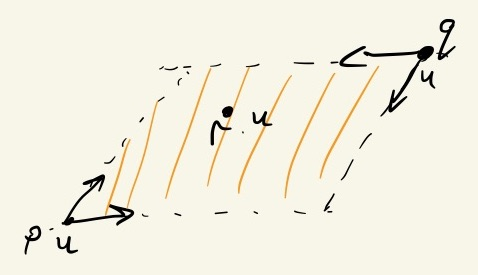
\includegraphics[scale=.5]{notes-21.jpg}}
    \caption{The points $p, q$ and $r$ described in proposition 1.}
  \end{figure}

  In the 3 dimensional inner algorithm, there were 2 possibilities for a down-set witness; top
  down-set witnesses and right down-set witnesses. With my pair there are 3 possible configurations,
  corresponding to the three faces of a cube adjacent to the top right corner. 

  \bibliographystyle{IEEEtran}
  \bibliography{notes}

\end{document}
